\chapter{相关研究综述}
\label{chap2}

\section{神经网络分布式训练}
目前神经网络在计算机视觉、自然语言处理与语音识别等多方面有着广泛的应用并取得了良好的效果,但是训练神经网络所需的计算量很大,对计算设备有着很高的要求。一台计算设备的计算能力有限,在面对参数较多的神经网络的训练时,训练时间会变得很长。为了加快神经网络训练速度,就需要使用多台计算设备进行分布式训练。

%可以放一个数据并行和模型并行的图,类似于https://blog.csdn.net/qq_35799003/article/details/84981009
神经网络主要有两种并行计算的方法,分别是数据并行和模型并行:
\begin{itemize}
    \item 数据并行是指每台机器上都有模型的一份副本,在每轮训练开始前,各个机器上的模型参数都是相同的。在每一轮训练中,不同机器获取数据集中不同的数据作为神经网络的输入,将各个机器的结果进行组合,更新各机器上的模型参数,并进行下一轮训练。
    \item 模型并行是指每台机器上都有一部分模型,不同机器负责不同部分的模型的计算。比如,以层为单位将神经网络分割并分配给不同的机器。
\end{itemize}

一般而言,数据并行是分布式训练的首选并行计算方法,因为数据并行不仅仅更容易实现,而且一般拥有更高的性能。本文主要关注数据并行。

数据并行的分布式训练需要在各个机器上的模型之间同步参数,其方法有很多种,我们只介绍最常见的一种同步方式---使用Allreduce算法进行模型参数的同步。

使用Allreduce算法进行模型参数同步的分布式训练大致过程如下:

\begin{itemize}
    \item [1)]
    每台机器上都启动分布式训练进程,对所有模型参数进行初始化。可以使用相同的随机种子与相同初始化方法来保证个机器中的模型初始化参数相同,也可以将某台机器中的进程作为主进程,由主进程初始化梯度,并通过Broadcast\footnote{Broadcast是MPI的一个原语(MPI\_Bcast),可以从一个进程读取数据,并且广播给通信域中的其他所有进程。}将参数广播给其他机器。
    \item [2)]
    每台机器从数据集中读取不同的数据作为输入。
    %可以放正向传播和反向传播的图片
    \item [3)]
    执行正向传播算法。神经网络的每一层根据当前层的输入进行计算,并将计算结果输出给之后的层。直到最后一层,算出最终结果,并与标定好的结果一起输入Loss Function(损失函数),得到Loss。
    \item [4)]
    执行反向传播算法。根据Loss,由深层至浅层,逐层计算出每个参数的梯度。
    \item [5)]
    调用Allreduce过程,将所有机器中参数的梯度逐元素求和并除以进程数以得到平均值。
    \item [6)]
    根据每个参数的平均梯度来对参数进行优化。由于各机器调用Allreduce后参数的平均梯度是相同的,调用的参数优化算法也是相同的,所以各机器间优化后的模型参数也依然是相同的。
    \item [7)]
    重复过程2)$\sim$6)的训练过程,直到手动终止训练或到达预设的训练轮数。
\end{itemize}

\section{模型裁剪}

相对于使用一台机器进行训练,分布式训练确实可以加速模型收敛,但是它的并行效率并不高,因为分布式训练需要调用Allreduce算法,而对于参数比较多的大模型而言,所有参数都需要输入Allreduce算法进行通信,由于网络带宽的限制,通信开销会非常大~\cite{li2014communication, wen2017terngrad}。

为了减少分布式训练中的通信时间,除了可以使用带宽更高的网络设备之外,还可以通过模型裁剪,减少通信量,以达到减少通信时间的效果。

出于压缩模型和减少分布式训练通信量的目的,模型裁剪得到了广泛的研究。在早期的研究工作中,模型裁剪能够大幅度降低模型复杂度并缓解过拟合的现象~\cite{lecun1990optimal, hanson1989comparing, hassibi1993second}。目前,模型裁剪的方法大多能够在不影响原网络模型精度的情况下,或多或少地降低分布式训练时的通信量,比如,设置一个阈值,只将大于这个阈值的梯度进行通信~\cite{strom2015scalable},或者降低梯度的精度以减少总通信量~\cite{seide20141}。

我们的工作是基于Yujun Lin等人的工作~\cite{lin2017deep},他们的研究表明,只需要将最重要的(也就是绝对值最大的)0.1\%的梯度进行通信,并配合动量修正和局部梯度裁剪,就能在大幅度降低通信量的基础上保持模型精度不变。

\section{MPI与Allreduce算法}
\label{section:MPI-Allreduce}
MPI的全称是Message Passing Interface,即消息传递接口,它是为高性能的大规模并行机器和工作站集群而设计的。MPI是一种标准接口,它有很多种实现,比如MPICH\footnote{http://www.mpich.org}和Open MPI\footnote{https://www.open-mpi.org}。MPI中包含很多原语,接下来介绍几种最基本且在神经网络分布式训练中需要用到的原语:
\begin{itemize}
    \item MPI\_Send与MPI\_Isend:通信集合中的一个进程向另一个进程发送消息。其中,MPI\_Send为阻塞式通信,而MPI\_Isend为非阻塞式通信。
    \item MPI\_Recv与MPI\_Irecv:通信集合中的一个进程从另一个进程接收消息。其中,MPI\_Recv为阻塞式通信,而MPI\_Irecv为非阻塞式通信。
    \item MPI\_Sendrecv:通信集合中的一个进程向另一个进程发送消息,并从另一个进程接收消息。
    \item MPI\_Barrier:阻塞程序继续执行直到通信集合中的所有进程都调用了这个函数。
    %可以加一个bcast的图
    \item MPI\_Bcast:通信集合中的一个进程向其他所有进程广播消息。
    %可以加一个allreduce的图
    \item MPI\_Allreduce:将通信集合中所有进程的缓冲区中的数值结合在一起,并将结果发送回所有进程。Allreduce支持多种运算符,比如使用加法运算符\footnote{由于神经网络分布式训练需要对梯度求平均值,所以需要用加法运算符。本文中默认Allreduce的运算符为加法运算符。},Allreduce就会将各进程的缓冲区中位置对应的元素相加。
\end{itemize}

MPI\_Allreduce的使用是神经网络分布式训练和单一计算设备上的训练的最主要区别。分布式训练需要通过Allreduce将所有进程的梯度求平均值,并用梯度的平均值来更新模型参数,以此来保证在每一轮训练之前各个进程中的模型参数是一致的。

Allreduce算法有多种实现方式,我们只介绍两种最常见的Allreduce算法:环形算法和蝶形算法。

%放一个环形算法的图
%放一个蝶形算法的图

\begin{figure}[ht] % use float package if you want it here
    \centering
    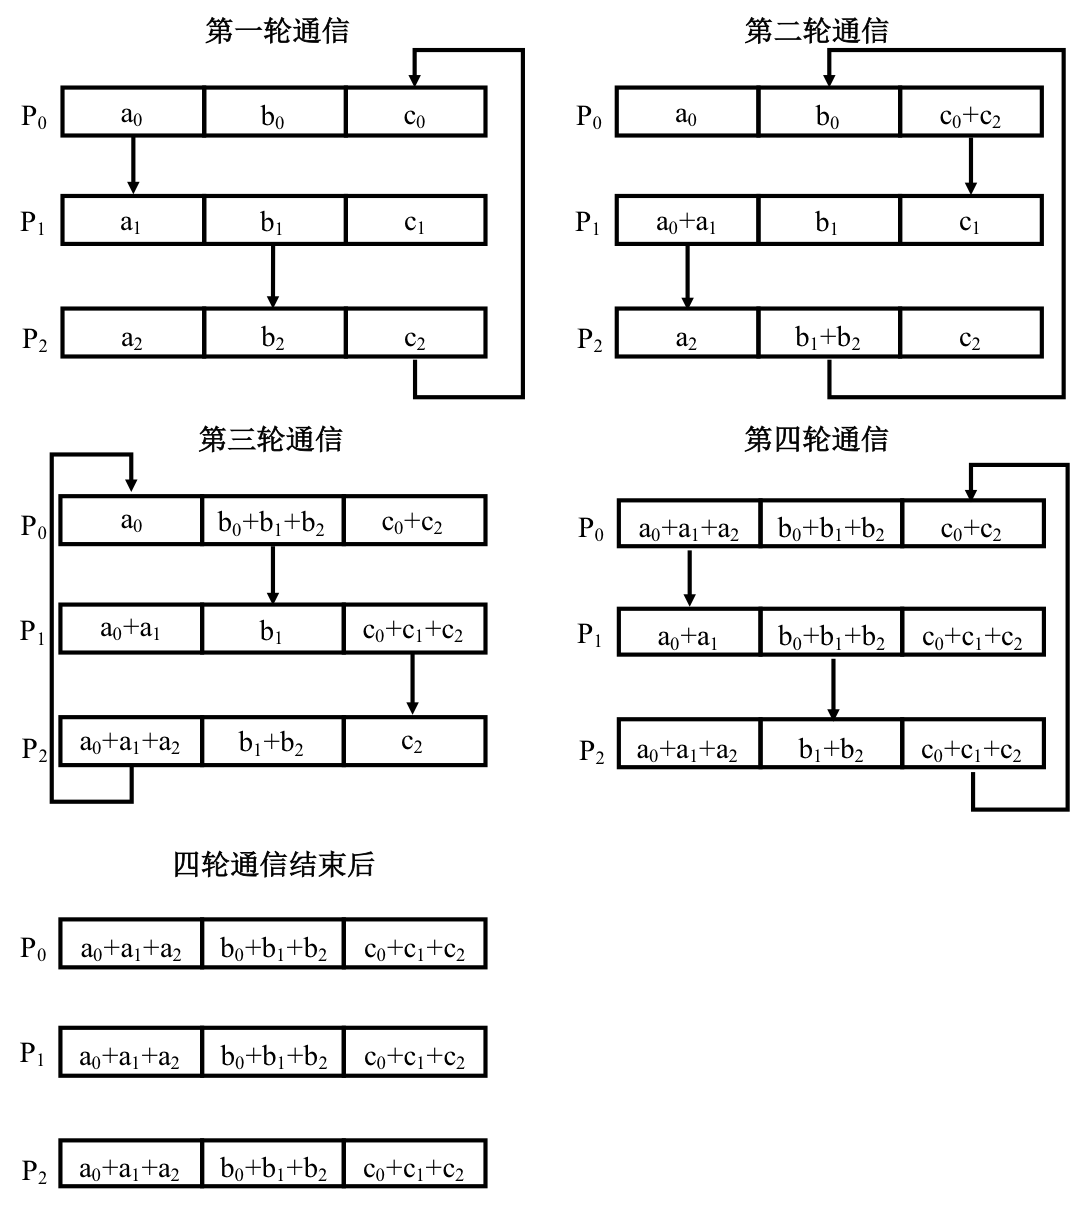
\includegraphics[width = 15cm]{ring-allreduce.png}
    \caption{环形Allreduce算法}
    \label{fig:ring-allreduce}
\end{figure}

\begin{figure}[ht] % use float package if you want it here
    \centering
    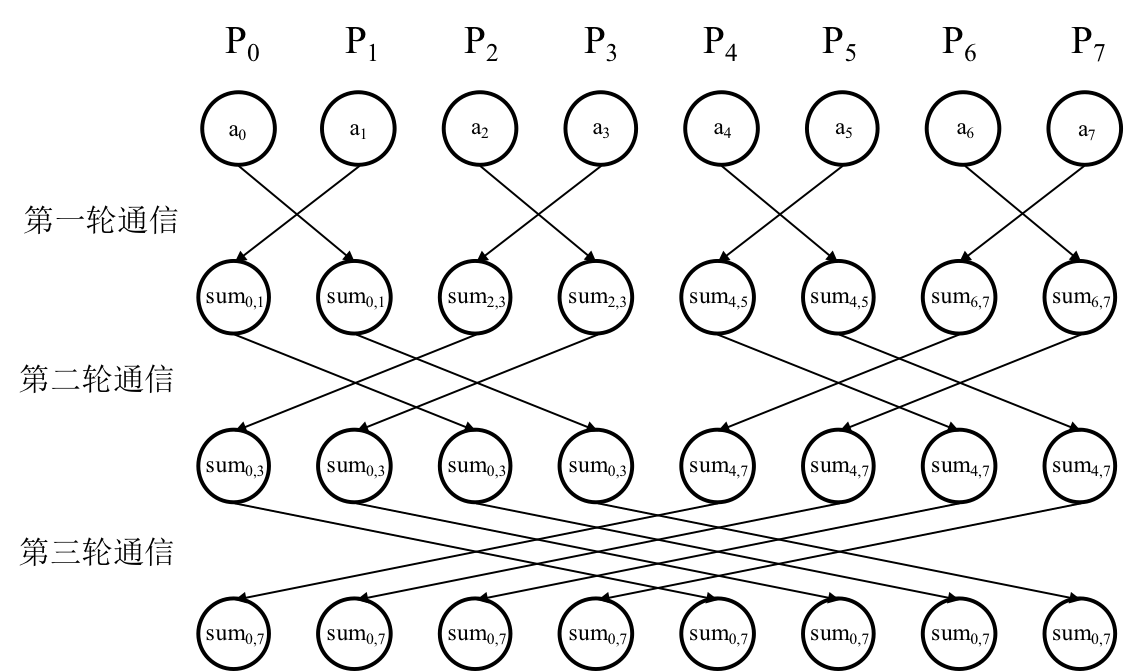
\includegraphics[width = 15cm]{butterfly-allreduce.png}
    \caption{蝶形Allreduce算法}
    \label{fig:butter-allreduce}
\end{figure}


环形算法与蝶形算法的示意图分别如图\ref{fig:ring-allreduce}和图\ref{fig:butter-allreduce}所示,其中,$sum_{l,r}$表示$\sum_{i = l}^r a_i$。环形算法具有通信总量少的优点,而蝶形算法具有通信轮数少的优点。两种算法的对比如表\ref{tab:Allreduce}所示。

\begin{table}[htb]
    \centering
    \caption[环形算法与蝶形算法对比]{环形算法与蝶形算法对比。P为进程数,L为缓冲区长度。通信量既包括发送量又包括接收量。只考虑P为2的整数次幂的情况。}
    \label{tab:Allreduce}
    \begin{tabularx}{\linewidth}{lXXX}
        \toprule[1.5pt]
        {Allreduce算法} & {通信轮数} & {单进程每轮通信量} & {单进程通信总量}\\\midrule[1pt]
        环形算法 & $2 \times P - 2$ & $\frac{2 \times L}{P}$ & $ \frac{4 \times (P - 1)\times L}{P}$\\
        蝶形算法 & $log_2(P)$ & $2\times L$ & $2 \times L \times log_2(P)$\\
        \bottomrule[1.5pt]
    \end{tabularx}
\end{table}

\section{随机选择算法}
有一类问题:给定一个包含n个数值的数组,需要从这n个值中选择出第k大的值。我们称此类问题为第k大值问题。在深度梯度压缩技术中,我们需要选择出绝对值最大的一部分梯度,这和第k大值问题是等价的,因为只需要选出第k大梯度,再找出比第k大梯度更大的梯度即可。

随机选择算法\cite{IntroToAlgo}可以在期望$\Theta(n)$的时间内解决该问题。

如同快速排序算法,随机选择算法的思想也是对输入的数组进行地规划分,不过与快速排序算法不同的是,随机选择算法只选择划分的一侧进行递归,而快速排序算法会在划分的两侧都进行递归。

以下是随机选择算法的伪代码,它返回数组a[l..r]中的第k大的元素。


\makeatletter
\newenvironment{breakablealgorithm}
  {% \begin{breakablealgorithm}
   \begin{center}
     \refstepcounter{algorithm}% New algorithm
     \hrule height.8pt depth0pt \kern2pt% \@fs@pre for \@fs@ruled
     \renewcommand{\caption}[2][\relax]{% Make a new \caption
       {\raggedright\textbf{\ALG@name~\thealgorithm} ##2\par}%
       \ifx\relax##1\relax % #1 is \relax
         \addcontentsline{loa}{algorithm}{\protect\numberline{\thealgorithm}##2}%
       \else % #1 is not \relax
         \addcontentsline{loa}{algorithm}{\protect\numberline{\thealgorithm}##1}%
       \fi
       \kern2pt\hrule\kern2pt
     }
  }{% \end{breakablealgorithm}
     \kern2pt\hrule\relax% \@fs@post for \@fs@ruled
   \end{center}
  }
\makeatother
%\begin{algorithm}[H]
\begin{breakablealgorithm}
\begin{algorithmic}[1]
\Procedure{RANDOMIZED-SELECT}{$a, l, r, k$}
\State $k \gets r - l - k + 2$
\If {$ l=r$}

\Return $a[l]$
\EndIf
\State $q \gets $ \Call{RANDOMIZED-PARTITION}{$a, l, r$}
\State $tmpK \gets q - l + 1$
\If {$ k = tmpK$}

\Return $a[q]$
\ElsIf {$k < tmpK$}

\Return \Call{RANDOMIZED-SELECT}{$a, l, q-1, k$}
\Else

\Return \Call{RANDOMIZED-SELECT}{$a, q+1, r, k-tmpK$}
\EndIf
\EndProcedure
\end{algorithmic}
%\end{algorithm}
\end{breakablealgorithm}

随机算法中调用了RANDOMIZED-PARTITION函数,它的作用是随机选择a[l..r]中的一个元素作为关键字,将比关键字小的元素都放在关键字左侧(下标小于关键字所在下标),其余元素放在右侧(下标大于关键字所在下标)。其伪代码如下所示,其中,RANDOM(i,j)表示从区间[i,j]中随机选取一个整数,SWAP(a[i], a[j])表示交换a[i]和a[j]的值.

\makeatletter
\newenvironment{breakablealgorithm2}
  {% \begin{breakablealgorithm}
   \begin{center}
     \refstepcounter{algorithm}% New algorithm
     \hrule height.8pt depth0pt \kern2pt% \@fs@pre for \@fs@ruled
     \renewcommand{\caption}[2][\relax]{% Make a new \caption
       {\raggedright\textbf{\ALG@name~\thealgorithm} ##2\par}%
       \ifx\relax##1\relax % #1 is \relax
         \addcontentsline{loa}{algorithm}{\protect\numberline{\thealgorithm}##2}%
       \else % #1 is not \relax
         \addcontentsline{loa}{algorithm}{\protect\numberline{\thealgorithm}##1}%
       \fi
       \kern2pt\hrule\kern2pt
     }
  }{% \end{breakablealgorithm}
     \kern2pt\hrule\relax% \@fs@post for \@fs@ruled
   \end{center}
  }
\makeatother
%\begin{algorithm}[H]
\begin{breakablealgorithm}
\begin{algorithmic}[1]
\Procedure{RANDOMIZED-PARTITION}{$a, l, r$}
\State $i \gets$ \Call{RANDOM}{$l, r$}
\State \Call{SWAP}{$a[r], a[i]$}
\State $x \gets a[r]$
\State $i \gets l - 1$
\For{$j \gets l$ to $r -1$}
\If{$a[j] <= x$}
\State $i \gets i + 1$
\State \Call{SWAP}{$a[i], a[j]$}
\EndIf
\EndFor
\State \Call{SWAP}{$a[i+1],a[r]$}
\State \Return $i + 1$
\EndProcedure
\end{algorithmic}
%\end{algorithm}
\end{breakablealgorithm}

\section{智能网卡}
智能网卡与标准网卡的主要区别在于智能网卡有相对较强的计算能力,它可以从主机端处理器卸载计算量。标准网卡的功能只有收发数据包、帧的拆封与封装等;而对于智能网卡而言,程序员可以在上面编程,使网卡可以处理更复杂的计算。

智能网卡主要基于两种技术解决方案,一种是现场可编程门阵列,另一种是中央处理器。

目前,智能网卡的主要应用包括数据包过滤(比如格式验证或分类),数据包转换(比如串行化、压缩或加密)、数据包引导(比如中央处理器核的负载平衡)以及数据包生成等。